\section{Materiais e Métodos}

\subsection{Descrição do problema}
No \ref{chap1} foi apresentado um problema magnético. Nele, um núcleo de chapas de aço era percorrido por um enrolamento que por sua vez era excitado com uma tensão à 60hz. Foram observados a densidade de fluxo magnético, o potencial elétrico e a intensidade de campo ao longo do núcleo magnético. O desenho do objeto, a definição dos materiais, a característica elétrica do circuito e outros parâmetros foram definidas no FEMM. Este capítulo apresenta o emprego da linguagem LUA para executar as tarefas realizadas na interface do aplicativo FEMM, conforme descrito no capítulo anterior.

\subsection{Comando para processar arquivo .LUA no FEMM}

\begin{figure}[h]
\centering
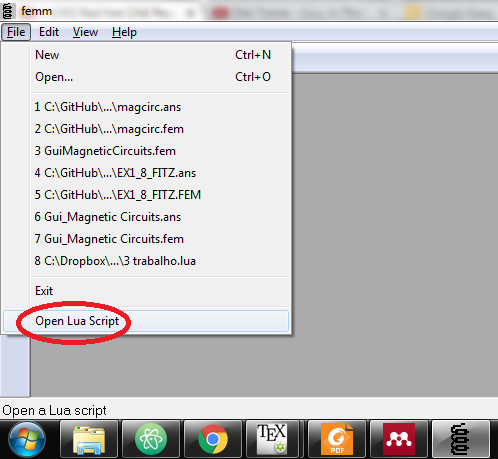
\includegraphics[scale=1]{img/assig2/open_lua_script.png}
\caption[Carregar arquivo script LUA]{Carregar arquivo script LUA.}
\label{circ}
\end{figure}
